\subsection{Description of the objective}

In the first step, only three entities are created: Alice, Bob and Charlie. The two peers need to read configuration files to know their own IP addresses. The tracker is not implemented yet, the client has to read a configuration file in order to know where the chunks are located.

Knowing the message format used in the project\footnote{\url{https://github.com/jpagex/elec-h-417-project/blob/master/statement.pdf}}, the peers will analyse the requests they receive from the client and they should be able to either send the chunk that was asked or to return an error message.

\subsection{Proposed solution}

Using object-oriented Python programming, classes \texttt{peers} and \texttt{client} have been created. Alice and Bob are thus \texttt{peers} objects and Charlie is a \texttt{client} object.

All the data transfer between the peers and the client are handled using TCP to ensure that every requested chunk is correctly transmitted (provided a peer owns it). Moreover, the code was designed to limit the opening and closing of sockets.

\subsubsection{Peers}

The way peers are implemented is quite straightforward. When instantiated, the peer opens a socket and stays idle while waiting for a connection. When a connection is received from the client, a single thread by peer is launched.

This thread will analyse the incoming messages and will send back the appropriate errors when necessary. If the message format and content is correct, the peer will send the requested chunk to the client.

The thread will run and send errors through the socket while there are incoming messages from the client. If the client stops communicating, the peer will assume that all the requests have been sent and it will close the connection.

\subsubsection{Client}

The client is implemented in order to achieve the maximum file transfer speed, while handling cases where the configuration file declaring which peer owns which chunk is not correct. Furthermore, the client works regardless of the number of peers.

Two threads are created so that the chunks are requested and downloaded from Alice and Bob in a parallel way. The library \texttt{Queue} is used, and four queues are created when the client is instantiated. The first and second queues contain the list of chunks that are only owned by one of the two peers (qA for Alice only and qB for Bob only). In this way, each thread is sending requests to a different peer and it is only asking for chunks that are not shared. When the queue associated to a thread is empty, it will request chunks that are owned by the two peers, which are listed in the third queue (qAB). The fourth (qtot) contains all the chunks needed. This implementation allows to ensure that if one the connections is slower that the other, the impact on the file transfer speed will be as little as possible.

Moreover, when a chunk which was placed in the queue qAB is not found where it was requested, it will be put in qA or qB, depending on which peer sent a \texttt{NOT FOUND ERROR}. This implies that the client will handle cases where the chunk is supposed to be owned by Alice and Bob but is actually owned only by one of the two.

\subsection{Sequence diagram}

A simplified version of the sequence diagram of the step 1 code is shown in Figure \ref{fig:step1}. It can be seen that the client uses two threads, each dedicated to the communication with one peer. The interactions with the second peer (Bob) are not shown for sake of clarity, since they are very similar to those concerning the first peer (Alice).

Three specific cases are described : 

\begin{itemize}
	\item Single chunk, no error : the thread gets the chunk to ask in the queue qA, which is filled with chunks only owned by Alice. It sends a request to the corresponding peer. If no error occurs, it writes the chunk on the disk and signals that the chunk was correctly received.
	
	\item \textit{Multi Chunk}, no error : the thread has finished to ask for chunks listed in qA, and is now getting them for the queue qAB, containing chunks that are supposed to be owned by both peers. The follow-up is the same as in the previous case.
	
	\item \textit{Multi Chunk}, \texttt{NOT FOUND} : if the thread is asking for a chunk listed in qAB but Alice responds that she does not actually own it, it is concluded that the other peer (Bob) owns it. It will thus add the given chunk in qB, so that the thread 2 will ask Bob for it.
\end{itemize}

\begin{figure}
	\centering
	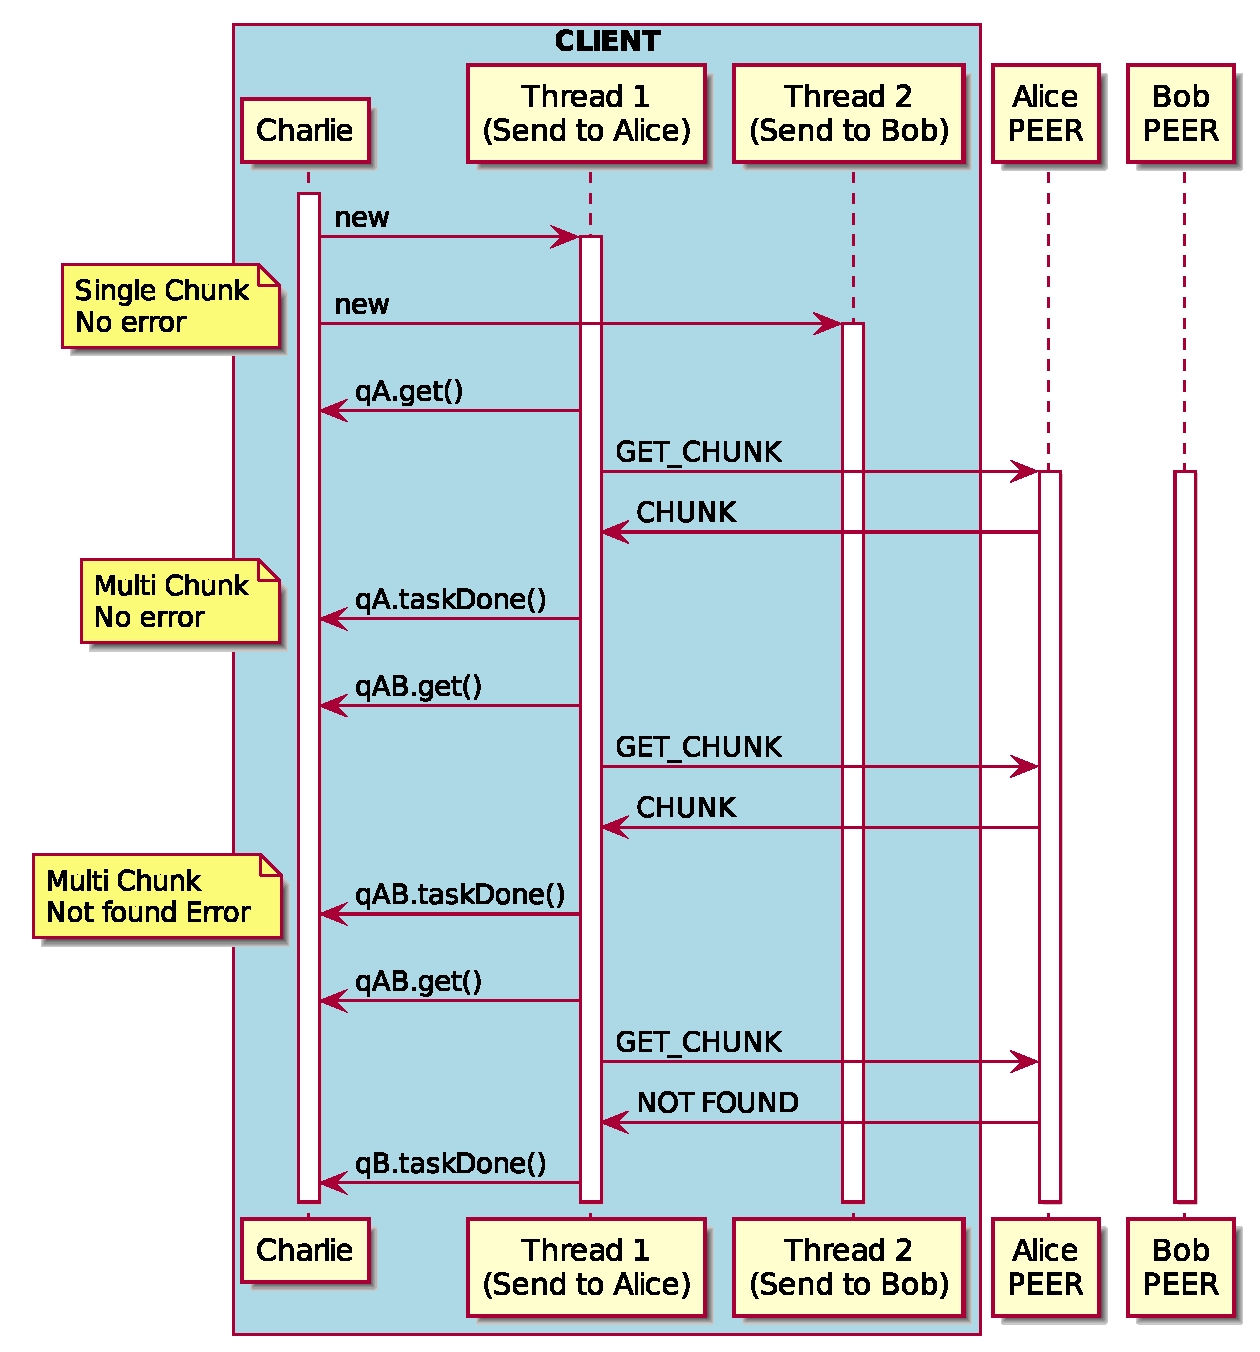
\includegraphics[width=\textwidth]{img/step1.eps}
	\caption{Sequence diagram of step 1}
	\label{fig:step1}
\end{figure}